\section*{\Large{АРХИТЕКТУРА СЕРВИСА}}
\addcontentsline{toc}{section}{АРХИТЕКТУРА СЕРВИСА}

На диаграмме размещения системы(см. рис\ \ref{pic:architecture__deployment-diagram})
расчетный сервис выделен голубым цветом.

\begin{figure}[H]
	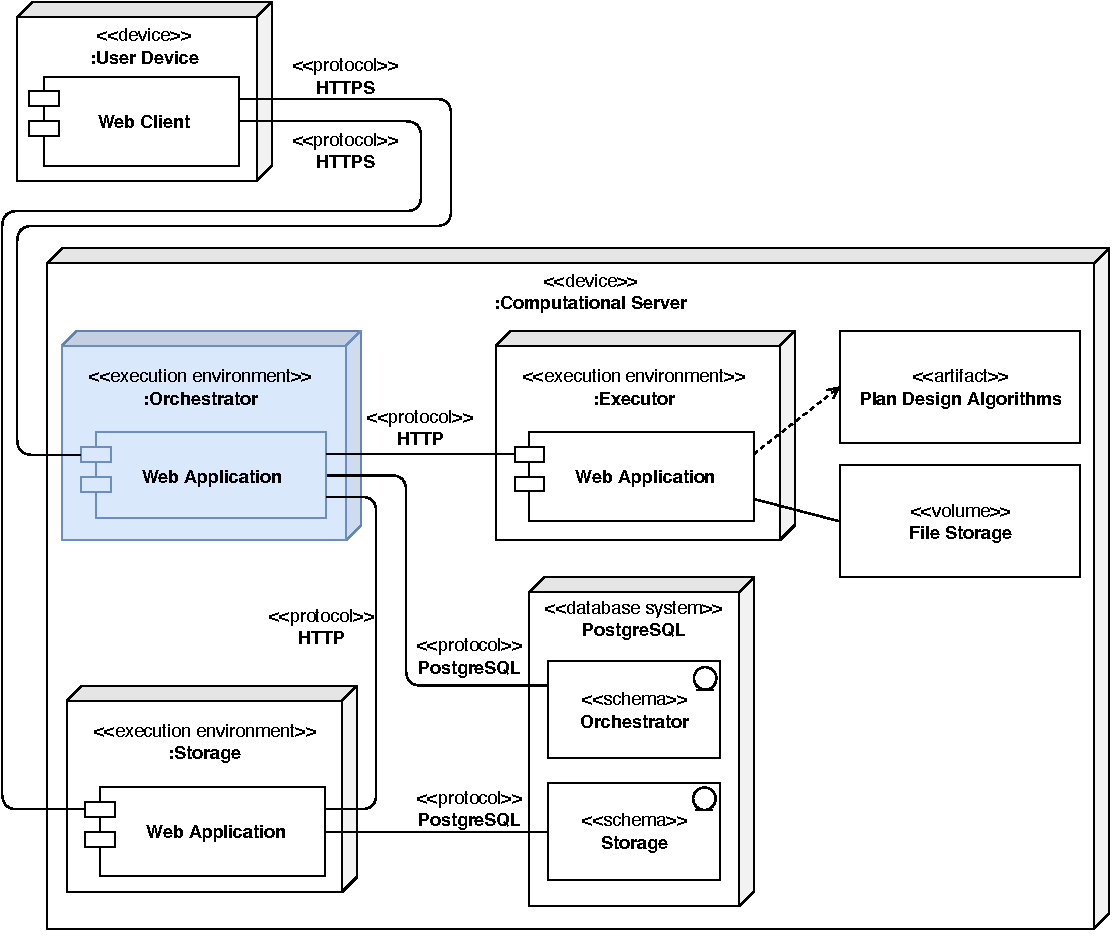
\includegraphics[width=\textwidth]{pictures/deployment}
	\caption{Диаграмма компонентов запуска расчётных задач}
	\label{pic:architecture__deployment-diagram}
\end{figure}
\vskip 5 mm


Архитектура сервиса запуска расчётных задач представлена на диаграмме
компонентов(см. рисунок \ \ref{pic:architecture__orchestrator-component}).

\begin{figure}[H]
	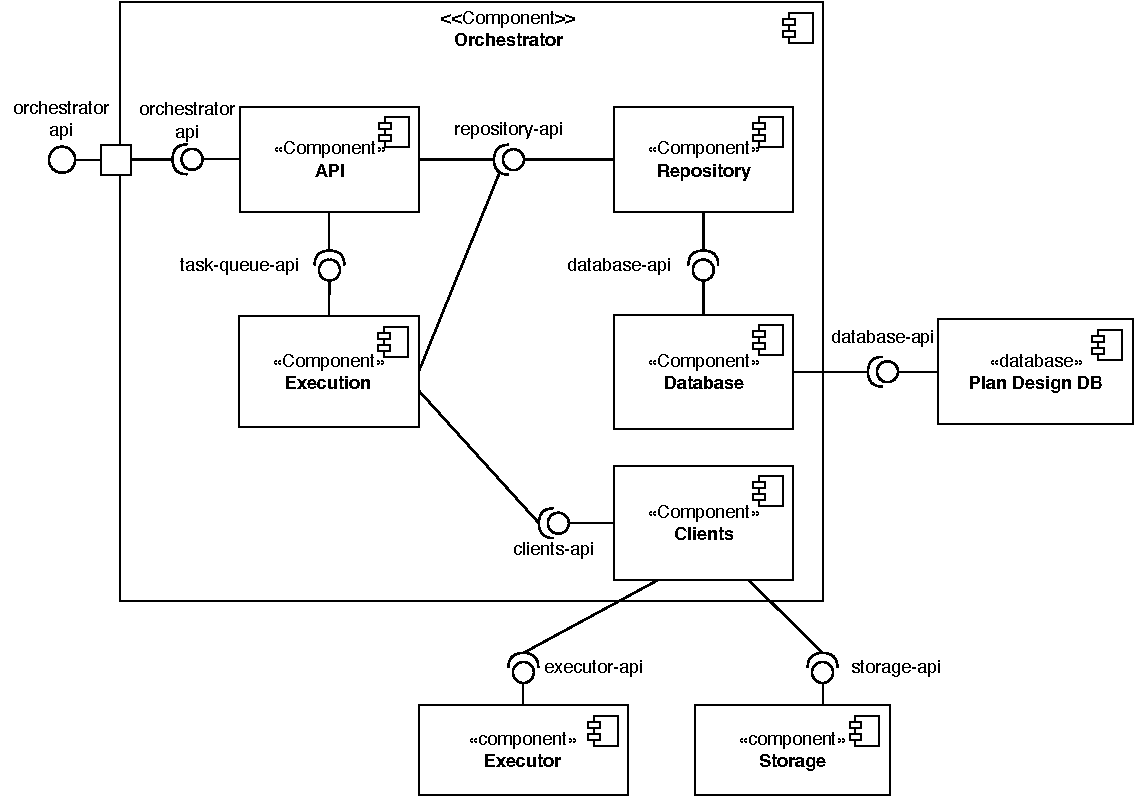
\includegraphics[width=\textwidth]{pictures/component_common}
	\caption{Диаграмма компонентов сервиса запуска расчётных задач}
	\label{pic:architecture__orchestrator-component}
\end{figure}
\vskip 5 mm

Сервис представлен следующими компонентами:
\begin{enumerate}
	\item {
		\textit{API} -- отвечает за предоставление REST API и отправки задачи в очередь.
	}
	\item {
		\textit{Repository} -- отвечает за получение и сохранение данных и логику их преобразований.
	}
	\item {
		\textit{Execution} -- компонент, отвечающий за выполнение расчётных задач.
	}
	\item {
		\textit{Clients} -- клиенты для взаимодействия с хранилищем расчётных данных
		и сервисом запуска математических методов.
	}
	\item {
		\textit{Database} -- чтение/сохранение сущностей базы данных.
	}
\end{enumerate}

Для расчёта генерального плана площадного объекта в автоматическом режиме используются четыре типа сущностей,
представленные на диаграмме ниже(см. рисунок .\ref{pic:architecture__orchestrator-classes})

\begin{figure}[H]
	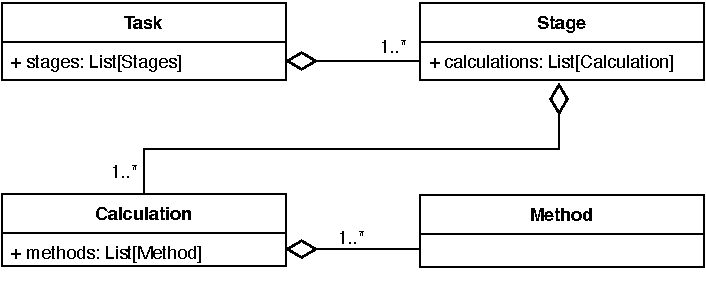
\includegraphics[width=0.8\textwidth]{pictures/classes}
	\caption{Диаграмма классов основных сущностей сервиса запуска расчётных задач}
	\label{pic:architecture__orchestrator-classes}
\end{figure}
\vskip 5 mm

\begin{itemize}
	\item {
		\textit{Task} -- расчётная задача.
		Результатом выполнения задачи является генеральный план площадного объекта.
		Задача состоит из набора этапов, выполняющихся строго последовательно.
		Результат выполнения следующего этапа зависит от результатов предыдущего.
	}
	\item {
		\textit{Stage} -- этап расчётной задачи.
		Для каждого этапа определен хотя бы один расчёт.
		Расчёты могут выполняться параллельно.
		Результатом этапа может быть только один расчёт.
	}
	\item {
		\textit{Calculation} -- расчёт. Состоит из последовательности методов.
	}
	\item {
		\textit{Method} -- метод. Способ применения математической методики.
	}
\end{itemize}

Такое разбиение на классы обусловлены высокой сложностью и вариативностью расчёта генплана.

Наименьшим блоком в расчёте генерального плана является метод. Метод является одним из способов применения
определенной математической методики, которая представлена в математической библиотеке.

Блок, который отвечает за последовательность вызова математических методик называется расчёт.
Для получения результата более высокого качества требуется иметь возможность последовательно выполнять несколько
математических методик.
Например, для того чтобы рассчитать правила минимальных допустимых расстояний с учётом зон теплового излучения
требуется вычислить параметры этих зон, а затем на основе полученных параметров произвести расчёт минимальных
допустимых расстояний. Таким образом последовательно вызываются две методики для получения одного расчётного элемента.

Объектом, который объединяет расчёты является этап. Этап состоит хотя бы из одного расчёта. В рамках этапа
расчёты могут выполняться параллельно. Входные данные расчёта зависят только от результата выполнения предыдущих этапов
задачи. Результатом этапа может быть только один результат расчёта.

Задача представлена набором этапов. Все этапы выполняются строго последовательно, результат последующего этапа
зависит от результата выполнения предыдущих.

Для оперирования с указанными сущностями предлагается следующая архитектура
компонентов(см. рисунок \ \ref{pic:architecture__orchestrator-detailed-component}).

\begin{figure}[H]
	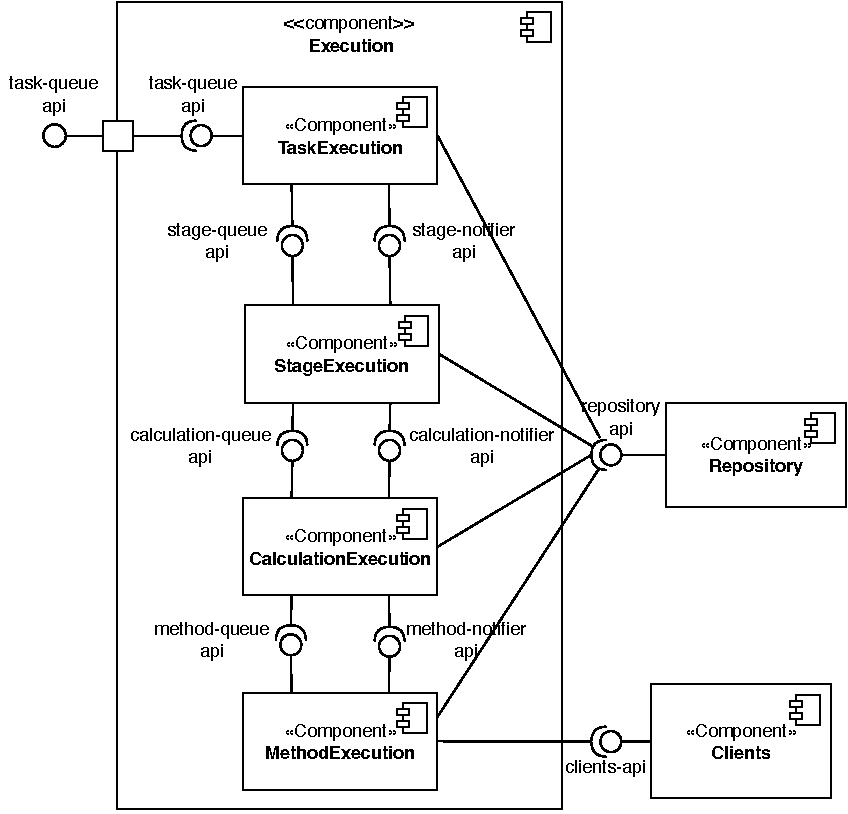
\includegraphics[width=\textwidth]{pictures/component_detailed}
	\caption{Диаграмма компонентов запуска расчётных задач}
	\label{pic:architecture__orchestrator-detailed-component}
\end{figure}
\vskip 5 mm

\begin{enumerate}
	\item {
		\textit{Task Execution} -- выполнение расчётной задачи.
	}
	\item {
		\textit{Stage Execution} -- выполнение этапа задачи.
	}
	\item {
		\textit{Calculation Execution} -- выполнение расчёта.
	}
	\item {
		\textit{Method Execution} -- выполнение математической методики.
	}
\end{enumerate}

\begin{figure}[H]
	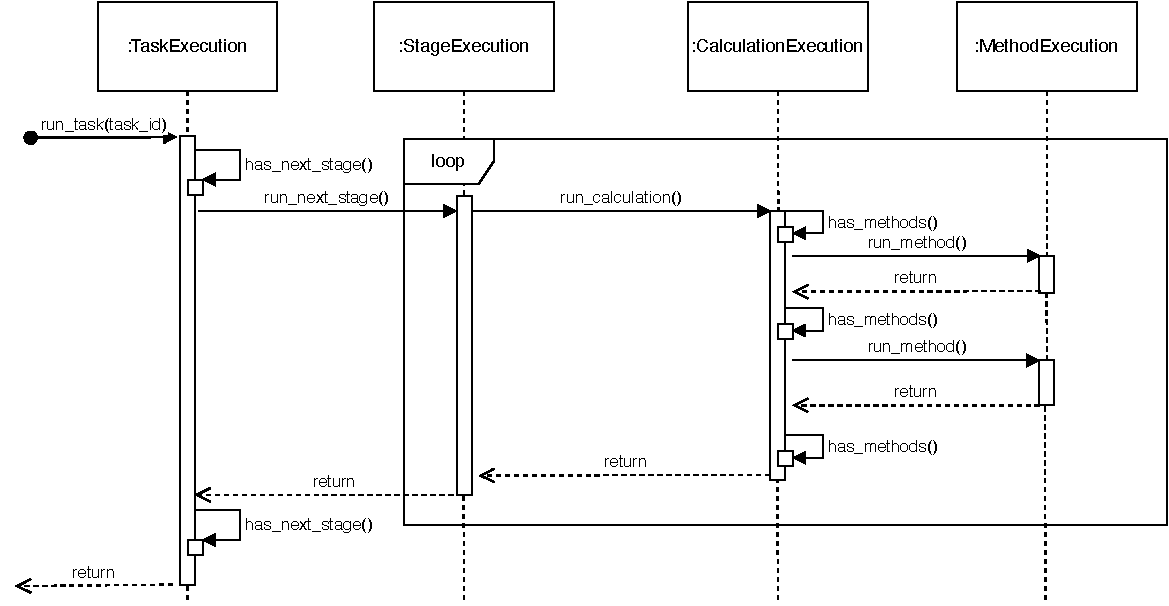
\includegraphics[width=\textwidth]{pictures/sequence}
	\caption{Диаграмма последовательности выполнения расчётной задачи}
	\label{pic:architecture__orchestrator-sequence}
\end{figure}
\vskip 5 mm

Выше представлена диаграмма последовательности выполнения расчётной
задачи(см. рисунок \ \ref{pic:architecture__orchestrator-sequence}).
Для её выполнения происходит вызов компонента \textit{TaskExecution}. Пока присутствуют
нерасчитанные этапы, происходит последовательный вызов компонента \textit{StageExecution}.
В рамках выполнения этапа расчётной задачи вызывается компонент, отвечающий за выполнение расчётов
\textit{CalculationExecution}.
Для выполнения одного расчёта последовательно вызывается компонент \textit{MethodExecution}.